\documentclass[12pt]{article}
\usepackage[english]{babel}
\usepackage[utf8]{inputenc}
\usepackage{blindtext, fancyhdr}
\usepackage{graphicx}
\pagestyle{fancy}

\title{Cut Detection Survey and Analysis for Long Form Video Game Streams \\ Prof. Prosenjit Bose}
\author{Jaime Herzog\\ 101009321 \\ jaimeherzog@cmail.carleton.ca}

\fancyhf{}
\rhead{\textit{\rightmark}}
\lhead{\textit{\leftmark}}
\rfoot{\thepage}

\begin{document}

\maketitle
\clearpage

\section{Abstract}
Shot Boundary Detection, or simply Shot Detection, is a fundamental part of research in the broader field of video analytics, used for essential video analysis tasks such as 
video indexing and content-based video retrieval. For professional video game live streamers, who create hours of continuous content with significant downtime, identifying
cuts in their streams is an important first step for automatically generating condensed stream highlights. In this project, I have summarized the nomenclature and methodologies
established in the academic canon for Shot Detection research, implemented a sample of the most common approaches, Colour Histogram comparison and Edge Change Ratio using Canny 
Edge Detection, and compared their effectiveness when used on video game live stream content, as well as establishing methodological challenges to this new content form.
\section{Acknowledgements}
Thank you to my project supervisor Professor Prosenjit Bose for his help and direction throughout this project.
\clearpage

\tableofcontents
\clearpage

\section{Motivation}
\subsection{Why Shot Boundary Detection?}
    With the proliferation of internet connectivity in recent years, there has been a massive increase in the volume of video on the internet.
With this growth, an industry built around the creation, hosting and sharing of video content grew as well, with YouTube alone having an annual revenue of over US\$15 billion
dollars~\cite{youtube}. Portable devices increase the accessibility for the creation and uploading of video content, and the combination of the 
massive social network surrounding content creation, with the enticing entertainment industry creating multi-millionaire content creators has 
exploded the sheer hours of video being uploaded daily. For YouTube, this type of content tends towards short-form video content at on average 10 minutes long. Comparing
this to video game live streamers, who in some cases are live 8 hours a day, 5 days a week, and in some cases even more frequently, the volume of video uploaded
per creator is significantly increased. In Q4 2019, there were 2.3 billion hours watched on Twitch, and 0.9 billion on YouTube Gaming~\cite{twitchusage}. 

    For live streamers, when they have so much continuous uptime, it is important to create highlights of their daily streams, in order to increase their reach to viewers who
don't have the time to watch their full time streams, as well as to diversify their brand onto a traditional YouTube channel. The creation of these highlights is extremely
time consuming, as the hours of content must be sifted through manually by either the content creators themselves, adding hours to their daily workload, or by hired editors. 
Commonly, it is unfeasable for streamers to spend all their spare time manually editing highlight videos for their daily streams, and for streamers with a lower viewerbase
and thus less income, it is also difficult to afford a full time editor. This creates another barrier of entry to the career of live streaming, a career track that is already
difficult to get started in due to the high viewership required for career viability. The solution for this currently manual labour is an automated editing system, which 
methodologically identifies key scenes and removes downtime. This could use some implementation of technology analogous to Story Segmentation, which was a task for TRECVID 2003
~\cite{storyseg}, or using representative key frame extraction. However, for anything like Story Segmentation or key frame extraction to be possible, it is essential that the
system first defines the video's scenes. To do this, we must find where scenes end, hence we use various shot boundary detection methods. 

\subsection{Cut Detection and Video Game Live Streaming}
    There has been siginificant research in the field of shot boundary detection over the past couple of decades, with multiple surveys of traditional shot detection methods
~\cite{lienhart1998comparison}~\cite{survey1}. The shot boundary detection is a fundamental part of the broader field of video segmentation, which refers to the partitioning 
of video into spatial, temporal, or spatiotemporal regions that are homogeneous in some feature space. Video segmentation itself is an essential part of many video analysis problems,
including, video summarization, indexing, retrieval, coding, authoring, and editing, as well as other applications in video surveillance and 3D motion and structure estimation with multiple
moving objects~\cite{bovik2009essential}. There are many different aspects of the shot boundary detection problem, due to the fact that shot boundary's are can be defined by multiple 
different types of scene transitions - either an abrupt cut, or a gradual transition, such as a fade or a dissolve. These different transitions have different properties and patterns 
(see figure 1) that the shot boundary detection system must analyze, usually with each type of transition analyzed independently. For the purposes of this project, we will implement
systems which detect abrupt cuts in video, and then apply these to systems to video game live stream clips.
\begin{figure}[ht]
    \centering
    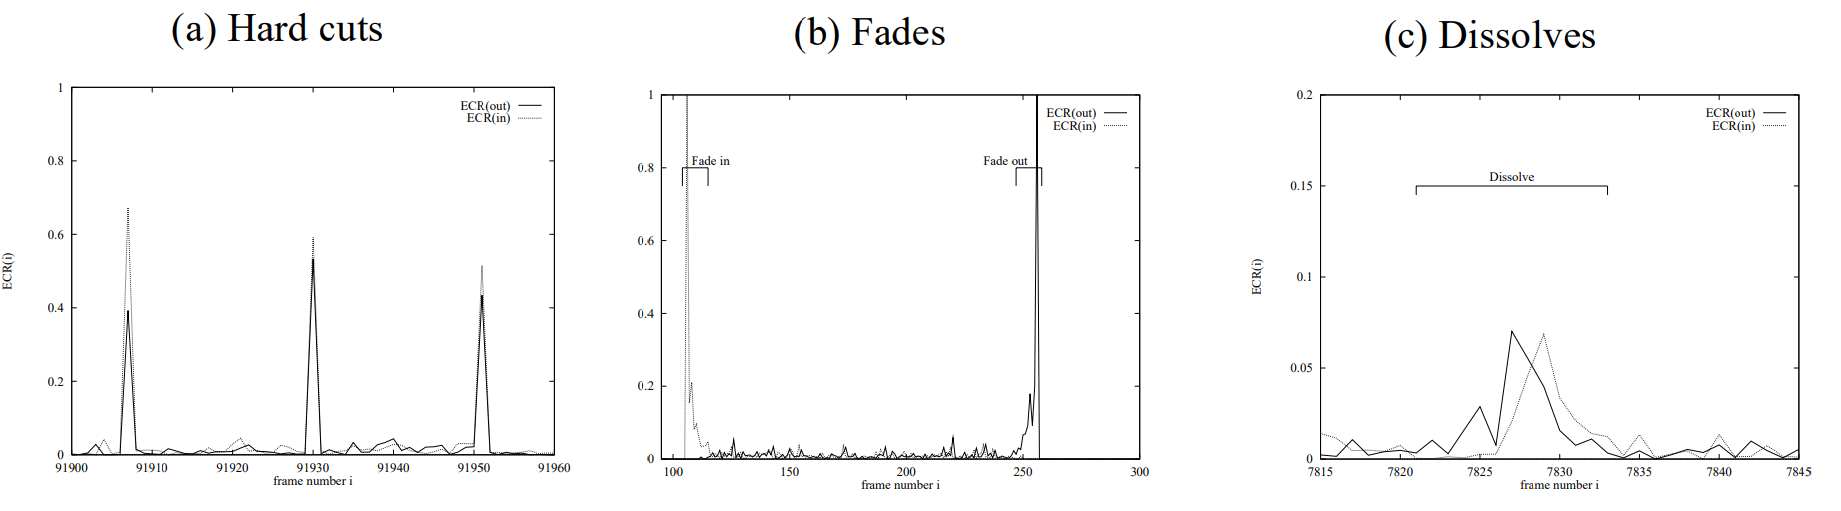
\includegraphics[width=1.0\textwidth]{fig1}
    \caption{Gradual Transitions: Their Differing ECR Values~\cite{lienhart1998comparison}}
    \label{Gradual Transitions}
\end{figure}

    Additionally, there has been as far as I know at the time of this project, no research on the topic of video game live stream cut detection. It is understandable why - the 
video game live streaming industry is still very young, and the change in domain when compared to more typical edited video or film is significant. Rather than there being a typical 
film or video editor defining the end of each scene, we must analyze and formulate the typical "scenes" that define contiguous activity in video game live streams. 
This project will examine the different possible approaches to defining scenes in video game live streams, and attempt to formulate a schema for which we can apply 
traditional cut detection techniques, as well as outline areas of potential new developments for specifically this area, similar to what has been done for sports television
video segmentation.
\clearpage

\section{Methodology}
\subsection{What is Video Game Live Streaming?}
Video game live streaming is the activity of a person recording themselves playing a game to a live audience. Popularized in the mid 2010s primarily on Twitch, it started
as just people who enjoyed playing games playing for people to build an audience and have fun playing games. By 2014, Twitch had more traffic than HBO's online streaming 
service~\cite{graziano_2014}, and it had begun to become more and more clear that the popularity of these live streams could generate significant revenue. As the community grew,
so did avenues of revenue for streamers, and before long there were more than a handful of video game livestreamers generating significant income, with many more able to make a 
living off of streaming full time.



Currently, the profession of video game live streaming is appealing to many, but ultimately extremely inaccessable. This is due to the fact that a streamer must have an 
established and loyal community which supports the streamer with paid subscriptions through Twitch, donations, or via Patreon. Other sources of revenue include:
\begin{itemize}
    \item Salaries from esports teams such as Cloud 9 or TSM, although these sponsorships are reserved for the most popular or skilled streamers. 
    \item YouTube channels which host short form highlight videos. The problem with this was touched upon in the Motivation section, but to emphasize, 
    it is very time consuming for streamers to manually curate highlights and create entertaining videos on top of streaming consistent hours to grow their 
    community, and for new streamers who have jobs on top of their streaming, this becomes an insurmountable barrier of entry.
    \item Sponsored content, such as a game studio paying a streamer to pay their game. Again, this type of revenue is only available to those select streamers
    who already have an established audience, as the paid content must be a viable investment to the sponsors.
\end{itemize}
This means that when a streamer is starting out, they must minimize their hours and keep a full time job, as it can take months or years before streaming 
income becomes viable full time. This leaves even less time for editing highlights of streams for increased reach, which further limits the accessibility, 
of building the brand necessary to be successful as a professional live streamer,  as discussed in the Motivation section.

\subsection{What is Shot Boundary Detection?}
We will begin by summarizing the problem of Shot Boundary Detection, and then we will take an overview of the formal schema for this problem as defined in Yuan et al.~\cite{survey1}
and how they must be modified to fit into the video game live stream content format.

Shot Boundary Detection is the broad problem of trying to build a system which automatically detects the beginning or end of a shot or scene, which for traditional 
film would be defined more precisely as an uninterrupted sequence of images captured by a single camera action. 
While the number of possible types of scene transitions is quite large, in practice, the vast majority of all transitions are either hard cuts, fades, or dissolves 
(at least when it comes to traditionally edited movies or video). 
\clearpage

\section{Results}
\blindtext
\clearpage

\bibliography{mybib}{}
\bibliographystyle{plain}
\clearpage

\end{document}